\documentclass[10pt,a4paper]{article}
\usepackage{researchsketch} % See researchsketch.sty %
\usepackage{enumitem}
\usepackage{algorithm}
\usepackage{algpseudocode}
\setenumerate[1]{itemsep=0pt, partopsep=0pt,topsep=5pt}
\setitemize[1]{itemsep=0pt, partopsep=0pt,topsep=5pt}
\author{1155189917}
\title{Theorems}
\pagestyle{fancy}
\renewcommand{\headrulewidth}{0pt}
\fancyhf{}
\rfoot{Page \thepage}
\date{\today}
\begin{document}
\noindent On Robustness of Quantized Neural Network Optimizations (Quantization-Aware Training)\hfill Findings\\
WONG, Hok Fong\hfill UG Summer Research Internship\hfill Last Updated: 21 Jul, 2024\\
\phantom{}\hrulefill

\section{Algorithm Descriptions and Proofs}
\setcounter{assumptioncnt}{0}
Consider the optimization problem $\min_{x\in C} f(x)$ where the feasible set $C=\{x\in \mathbb{R}^n \bigm| g(x)\geq 0\}$, the objective function $f:\mathbb{R}^n\rightarrow \mathbb{R}$, and the constraints are described by the function $g: \mathbb{R}^n \rightarrow \mathbb{R}^d$.

\assumption{
     The functions $f$, $g$ are continuously differentiable and have a Lipschitz continuous gradient. $f(x)\to \infty$ when $\lvert x\rvert \to \infty$ and $C$ is non-empty and bounded.
}

\assumption{
     The Mangasarian-Fromovitz constraint qualification (MFCQ) is satisfied for all $x\in \mathbb{R}^n$, i.e. $\forall x\in \mathbb{R}^d$, $\exists w\in \mathbb{R}^n$ s.t. $\nabla g_i(x)w>0$ for all $i\in I_x$, where $I(x)=\{i\in \mathbb{Z}\bigm| g_i(x)\leq 0\}$.
}

\noindent\textbf{Fact.} The MFCQ condition is automatically satisfied for $x\in C$.

Tangent cones have a natural role in the theory of flow-invariant sets and gradient inclusions.

\definition{
     The Clarke's tangent cone of $C$ contains all $\delta x\in T_C(x)$ if there exists two sequences $x_j\rightarrow x, x_j \in C, t_j\downarrow 0$ such that $(x_j-x)/t_j\rightarrow \delta x$. The normal cone is defined as follows: $N_C(x)=\{\lambda\in \mathbb{R}^n\bigm| \lambda^{\top}\delta x\leq 0, \forall \delta x\in T_C(x)\}$.
}

\lemma{
     Suppose that $x\in C$, then every $\delta x\in T_C(x)$ satisfies $\nabla g_i(x)\delta x\geq 0, \forall i\in I_x$. The converse also holds.
}

\begin{proof}
     $(\Rightarrow):$ $\delta x\in T_C(x)$ implies that there exists two sequences $\{x_j\}\rightarrow x, \{x_j\}\subset C, t_j\downarrow 0$ for all $j\in \mathbb{N}$ and $$\frac{x_j-x}{t_j}\rightarrow \delta x,$$ which implies that $$\frac{g(x_j)-g(x)}{x_j-x}\cdot\frac{x_j-x}{t_j}\geq 0.$$ This is because $x_j\in C$ implies that $g_i(x_j)\geq 0$ and $g_i(x)\leq 0$ for all $i\in I(x)$.

     $(\Leftarrow):$ Adapted from R. Herzog, 2023, a simplified version. Let $\delta x$ satisfy $\nabla g_i(x)\delta x\geq 0, \forall i\in I_x$, also let $\delta y$ be given by MFCQ such that $\nabla g_i(w)\delta y>0, \forall i \in I(x)$. Put $\ell(t):=\delta x+ t\cdot\delta y$. Then for all $t>0$, we have $\nabla g_i(x) \ell(t)>0, \forall i\in I(x)$, implying that $\ell(t)$ are all feasible MFCQ vectors.

     Now, we claim that $\ell(t)\in T_C(x)$ for all $t\in \mathbb{R}_{++}$. Let $\gamma(t):=x+t\ell(t)$, $t\in(-\eps, \eps)$, for an infinitestimally small $\epsilon$, given by the continuity of $g$. Then, $y(t)\in C$ for every $t\in [0, \epsilon)$ and $\gamma(0)=x, \gamma'(0)=\ell(t)$. For an arbitrary sequence $\{t_j\}\downarrow0$ and $x_k = \gamma(t_j)\rightarrow x$ we have $$\ell(t)=\gamma'(0)=\lim_{j\to\infty} \frac{\gamma(t_j)-\gamma(0)}{t_j-0}=\lim_{j\to\infty}\frac{x_j-x}{t_j}\in T_C(x).$$

     Since $T_C(x)$ is closed, $\delta x=\lim_{t\to0}\ell(t)\in T(x)$.
\end{proof}

Now, we can simplify the tangent cone and the normal cone for any $x\in C$ as follows, due to the Mangasarian-Fromovitz constraint qualification: $$T_C(x)=\{x\bigm|\nabla g_i(x)^{\top} x\geq 0, \forall i \in I_x\}, N_C(x)=\left\{\lambda\in \mathbb{R}^d_{+}\middle|-\sum_{i\in I(x)} \lambda_i \nabla g_i(x)\right\}.$$

\definition{
     Further define the set $V_\alpha(x):=\{v\in \mathbb{R}^n\bigm|\nabla g_i(x)^{\top}v+\alpha g_i(x)\geq 0, \forall i \in I_x\}$, where $\alpha>0$. $V_\alpha(x)$ is guaranteed to be non-empty for any $x$.
}

Indeed. For the case where $x\in C$, $V_\alpha(x)$ is nothing but $T_C(x)$. Otherwise, consider any $g_i(x)<0$, by MFCQ there exists $u$ such that $\nabla g_i(x)^{\top} u> 0$ and therefore by scaling we have $\nabla g_i(x)^\top v\geq -\alpha g_i(x)\geq 0$.

\definition{
     The indicator function for a set $C$ is defined as:

     $$\psi_C(x)=\begin{cases}
               0,      & x\in C,           \\
               \infty, & \text{otherwise}.
          \end{cases}$$
}
\theorem{
Let $x:[0, \infty)\rightarrow \mathbb{R}^n$ be an absolutely continuous trajectory with a piecewise continuous derivative. Then, for any $x(0)\in C$, the following are equivalent:

$$\begin{aligned}
           & \dot{x}(t):=-\nabla f(x(t))+R(t), -R(t)\in N_C(x(t)),                                           &  & \forall t\in [0, \infty) \text{ almost everywhere}, \\
           & \dot{x}(t)^+:=-\nabla f(x(t))+R(t), -R(t)\in \partial\psi_{V_\alpha(x(t))}(\dot{x}(t)^+),       &  & \forall t\in[0, \infty),                            \\
           & \dot{x}(t)^+:=-\argmin_{v\in V_{\alpha}(x(t))}{\frac{1}{2}\abs{v+\nabla f(x(t))}^2}, \phantom{} &  & \forall t\in[0,\infty).
     \end{aligned}$$
}

\lemma{Using the \texttt{ASkewSGD} algorithm with step sizes $\{\gamma_k\}$ of $\sum_{i=1}^\infty \gamma_i=\infty$, $\sum_{i=1}^\infty \gamma_i^2<\infty$, the iterate $\{w_k\}$ is guaranteed to converge and $\lim_{k\to\inf} d(w_k,C_\epsilon)=0$.}

\begin{proof}
     See Leconte et al., 2023, Appendix A.3.
\end{proof}

\lemma{Let $k_0=\sup_{1\leq i\leq d,1\leq j\leq K_i}\sup\{k:\gamma_kM\geq\max(c_- - \frac{c_j^i+c_{j+1}^i}{2},-c_+ + \frac{c_j^i+c_{j+1}^i}{2})\}$. Since $w$ must }



\newpage
% \section{Derivation of Distance between $w$ and $C_\varepsilon$}


\section{Piecewise Convexity}

The piecewise convexity can be granted given the changes applied to the constraints.

\definition{
A function $F: \mathbb{R}^n \mapsto \mathbb{R}$ is called a piecewise convex function on $\mathbb{R}^n$ if it can be decomposed into:
$$F(x) = \min\{f_1(x), f_2(x), \ldots, f_m(x)\}$$
where $f_j: \mathbb{R}^n \mapsto \mathbb{R}$ are convex functions for all $j \in M = {1, 2, \ldots, m}$.
}

\lemma{
     Given a set of $K$ quantization levels $\mathcal{Q}=\{q_1, q_2, \ldots, q_K\}$. Define the piecewise function $$\psi(w):=\begin{cases}(q_{1}-w),& w < q_{1},\\(q_{i-1}-w)(w-q_{i}),& q_{i-1}\leq w < q_{i}, i=2,\ldots, K\\w-q_{K},& w \geq q_{K},\end{cases}$$ for all $w\in\mathbb{R}$. Then, $-\psi'$ is a piecewise convex function.
}
\begin{proof}
     That is, to prove that $\psi$ can be decomposed into concave functions $f_1, \ldots, f_m$ where $F(x)=\max(f_1(x), f_2(x), \ldots, f_m(x))$.

     \begin{center}
          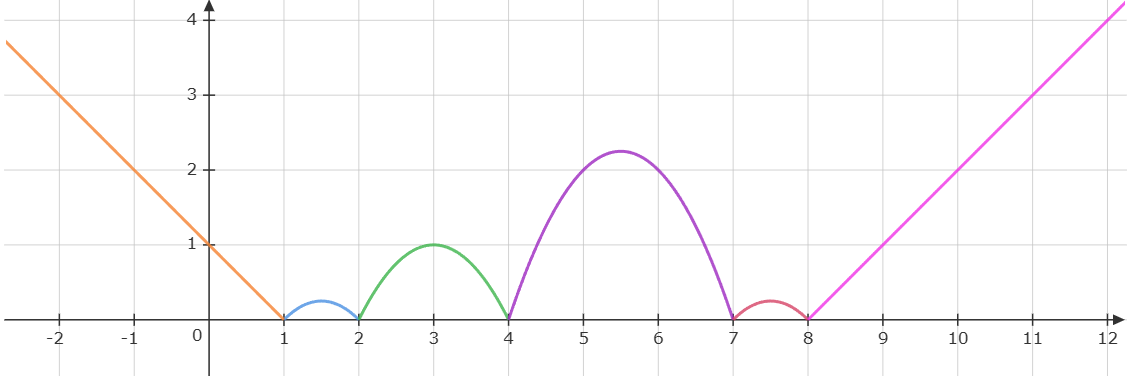
\includegraphics[width=0.5\linewidth]{psi.png}
     \end{center}

     The proof is pictorially shown by the plot above. Select $m=K+1$ such that the $f_i$'s $(i=1, \ldots, K+1)$ corresponds to the analytic continuation of every piece of function.

     $$\begin{cases}f_1(w):=(q_{1}-w),\\f_{i}(w):=(q_{i-1}-w)(w-q_{i}), i=2,\ldots, K\\f_{K+1}(w):=w-q_{K}.\end{cases}$$
\end{proof}

\textbf{Note.} We have changed the definition of $\psi$, the preliminary verification through proofs shows no problem of convergence failure. Apparently the new setup still satisfies the MFCQ condition for every $w\neq (q_i+q_{i+1})/2, \forall i=1, \ldots, K-1$. Also observed that this change does not alter the convergence property for the logistic regression problem. Now, we should note that $$0<\varepsilon\leq \inf\limits_{1\leq i\leq d}\inf\limits_{1\leq j\leq K^i} \abs{c_j^i-c_{j+1}^i}^2/4$$ ensures the disconnectedness of the set $C_\eps$.

\newpage
\section{Lagrange Duality}
\noindent The problem $\mathcal{P}$ of $$\min\limits_{x\in C} f(x), C=\{x\in \mathbb{R}^n\bigm| g(x)\leq 0\}$$ is equivalent to the primal problem $$\inf\limits_{x\in \mathbb{R}^n}\sup\limits_{\lambda\succeq 0} f(x)+\sum\limits_{i=1}^d \lambda_i g_i(x).$$ We consider the dual problem $$\sup\limits_{\lambda\succeq 0}\inf\limits_{x\in \mathbb{R}^n} f(x)+\sum\limits_{i=1}^d \lambda_i g_i(x).$$

\theorem{
     Suppose that $x^{*}$ is a local minimizer of $\mathcal{P}$ which satisfies the MFCQ. Then there exist Lagrange multipliers $\lambda^*$ (not necessary unique) such that the KKT conditions are satisfied. The set of Lagrange multipliers $\Lambda(x^*)$ is compact.
}

Therefore, the KKT points can be captured by the following set: $$\mathcal{Z}_\eps=\{w\in C_\eps: 0\in -\nabla \ell(w)+N_{C_\eps}(w)\}$$

\theorem{
     If $f: \mathbb{R}^d \mapsto \mathbb{R}$ is twice continuously differentiable and satisfies the strict saddle property, then gradient descent with a random initialization and sufficiently small constant step size converges to a local minimizer or negative infinity almost surely. Call $x$ a critical point of $f$ if $\nabla f(x) = 0$, and say that $f$ satisfies the strict saddle property if each critical point $x$ of $f$ is either a local minimizer, or a “strict saddle”, i.e, $\nabla^2 f(x)$ has at least one strictly negative eigenvalue.(J. D. Lee, in PMLT, 2016)
}

% Define the function $f^i_j(w) = -\varepsilon + \psi^i_j(w)$ for $j=1,2,\ldots, K+1$, and $i$ stands for the $i$-th parameter of the model.

\begin{algorithm}
     \caption{Dual gradient ascent method (convex constraints)}\label{alg:cap}
     \begin{algorithmic}[1]

          \State Start with an initial dual guess $\lambda(0) \geq 0$.
          \For {$k=1, 2, \ldots$}
          \State $x^{(k)}\in \argmin\limits_{x} \ell(x)+(\lambda^{(k-1)})^{\top}g(x)$
          \State $\lambda^{(k)}=\max\{\lambda^{(k-1)}+\gamma_kg(x^{k}), 0\}$
          \EndFor
     \end{algorithmic}
\end{algorithm}

\assumption{
     The objective function $f$ is convex and continuously differentiable.
}

How we can find $x^*$ efficiently, as $\nabla \ell$ is implicit? % Pointed out that, it may be difficult to evaluate the dual (requires unconstrained minimization of Lagrangian). We can consider coordinate-wise descent but 

The problem is that $f(x)-\mathbf{\lambda}g$ is a combination of a convex and a concave function (where $g$ is convex and $g\geq 0$ is required).

\url{https://proceedings.neurips.cc/paper_files/paper/2023/file/a961dea42c23c3c0d01b79918701fb6e-Paper-Conference.pdf}

% \theorem{
%      Given convex, differentiable $f: \mathbb{R}^n \to \mathbb{R}$, if we are at a point $x^*$ such that $f(x^*)$ is minimized along each coordinate axis, then $x^*$ is a global minimizer, i.e. $f(x+\delta e_i)\geq f(x)$ for all $\delta, i$ leads to $f(x)=\min_z f(z)$.
% }


% Now we consider the subroutine of finding $x^{(k)}$ by the coordinate descent algorithm.

% Even though we have assumed convexity of the loss function $\ell$, the new algorithm is novel in the sense that:

% \begin{itemize}
%      \item New edits to the constraint function $\psi$ with piecewise convex properties.
%      \item We can precisely control the error bound of our weights by $\varepsilon$.
%      \item The annealing step is unnecessary - thus lowering the time complexity.
%      \item The function can be non-smooth, as long as convexity is guaranteed (Sub-gradient methods, and see Nesterov, 2012).
% \end{itemize}

% We also notice some limitations of our proposed method:

% \begin{itemize}
%      \item The algorithm cannot be extended to equality constraints due to the simultaneous minimization of multiple quantization constants.
%      \item The algorithm's complexity is determined by the quantization levels, with small tolerance of interval size.
% \end{itemize}


\newpage
\section{Discussions}

\subsection{More ideas}
Under the assumption of non-summable and square-summable step sizes, $\lim\sup_{k\to\infty} d(w_k, C_\epsilon)=0$ almost surely. Given that the current piece $C_\epsilon$ is convex, disconnected, can we guarantee that $d(w_k, \mathcal{Z}_{\epsilon})$ converges almost surely? Note that the direction picked by speed never guide $w$ to leave the feasible set if any constraint is already violated.  (Will continue to read Boob, 2019. \textit{arXiv}: \url{https://arxiv.org/pdf/1908.02734})

First, we want to know if the algorithm escapes from saddle points (so not just stationary points but minimizers). (Stochastic case follows from \url{https://sites.math.washington.edu/~ddrusv/aiming_deep.pdf} and \url{https://hal.science/hal-03442137/file/tame.pdf}, step sizes \url{https://hal.science/hal-02564349/file/clarke.pdf})

Second, yet another Gradient Flow inspection. (\url{https://openreview.net/pdf?id=xuw7R0hP7G})

Third, experiment on C1-smooth and non C2-smooth functions (don't really know if they are even usable). Example: finding out the cases when the algorithm fails to converge?

Fourth, another algorithm for non-convex optimization. (\url{https://arxiv.org/pdf/1908.02734})

\subsection{A survey of quantization methods}

\subsection{Updates on the numerical experiment}

\subsection{Incoming Events}

\end{document}
